\documentclass[12pt]{book}
\usepackage[british]{babel}
\usepackage[utf8]{inputenc}
\usepackage{amsmath}
\usepackage{graphicx}
\usepackage{parskip}
\usepackage{natbib}
\usepackage{pgfgantt}
\usepackage{lscape}
\usepackage{pdfpages}
\usepackage{graphicx}
\usepackage{xcolor}
\usepackage[minted]{tcolorbox}
\usepackage{hyperref}
\usepackage[chapter]{tocbibind}
\usepackage[a4paper,vscale=0.85]{geometry}
\usepackage{doc}

\title{Project Terms of Reference -- A project example}
\author{Alun Moon}

\begin{document}
\frontmatter
\begin{titlepage}
    Thesis
\end{titlepage}

\newpage
Dedication

\newpage
Declaration

\tableofcontents

\mainmatter
\chapter{Introduction}
%!TeX root=Dissertation.tex

Hello

\part{Analysis}

\part{Synthesis}

\part{Evaluation}


\bibliographystyle{plainnat}
\bibliography{c,unix,writing,latex}

\part{Appendices}
\appendix

\chapter{Terms of Reference}
\pdfminorversion=4
\documentclass[]{article}
\usepackage[utf8]{inputenc}
\usepackage{amssymb,latexsym,amsmath}
\usepackage[a4paper,top=3cm,bottom=2cm,left=3cm,right=3cm,marginparwidth=1.75cm]{geometry}
\usepackage{graphicx}
\usepackage[colorlinks=true, allcolors=blue]{hyperref}
\begin{document}

%!TeX root=TermsOfReference.tex
\title{KV6003: Individual Project\\ Project Terms Of Reference}
\author{Cuthfbert Mutumbwa\\ Design and Implement a Rendering Engine}
\date{\today}

\maketitle

\section{Background}
Creating A rendering engine is a task that requires one to understand multiple different topics and subjects, for example not only will I need to know how lighting works, but how it interacts with other objects, and how to represent it on screen. I will also need to learn how textures work, how to wrap them around an object and how the light will interact with the texture wrapped around the object.
I will also learn how a modern GPU, by writing code for it, as well as understand what role the CPU will have when drawing the 3D images.
\\\\
In college, I used two pieces of software that are called Unreal Engine and Blender. Unreal Engine was a game engine, and Blender was a 3D Creation suite that can be used as a rendering engine.
My first question when using this software where "How does one Create 3D graphics software", then I realized I also was unsure of how someone designs this software.
\\
I want to create a rendering engine that uses core rendering techniques and features, and Software engineering practices to design the engine. for the design aspect, I have opted to use different types of literature such as Designing a Modern Rendering engine \cite{designengine} to help me.  I will also literature to choose which type of technique I will use to implement my features, this is because there are multiple different ways to implement features such as shadows, lighting, and even the way the engine will render a scene.
\\\\
Rendering engines are still or more specifically rendering is a very interesting field of study. New rendering features are being made to improve quality in 3D animated films, and recently Nvidia released a new Graphics Card to allow Real-Time raytracing in Video Games\footnote{\url{https://www.pcgamer.com/uk/what-is-ray-tracing/}}. Such an Achievement is one that is truly impressive as raytracing is known for being computationally expensive. 
\\\\
Creating a rendering engine is not only about knowing how to write good and efficient code, and knowing how lights, shadows, and texturing works are not enough. I will need to understand the underlining mathematical principles of computer graphics such as vectors, matrices and more. I will need to be able to read mathematical notation, as well as choose which formulas I will use to achieve the results I want.
I want to improve my mathematical skills, as well as know, learn what types of maths is needed to achieve this I have picked out literature and books such as  Game Physics Cookbook \cite{gamephysics}. This book teaches the reader the maths needed to make the rendering engine.
\\\\\\\\\\\\
\section{Proposed Work}
For the design phase I will use UML diagrams to help me conceptualize the rendering engine, and use them as a reference when creating the product. I will also incorporate a software Development life cycle to allow me to justify my choices, and allow me to see if I am on track to finishing the product.
I will create a 3D scene environment that will showcase the features I plan on implementing. The user will be allowed to freely move around the 3D scene environment. The user will see different showcases on features within this scene, for example, there may be a location where the user is able to an object reflection from another object, and a location that demonstrates shadows by casting a light above the object.
\\\\
Since there are many types of ways to implement one feature, in my design phase I have to consider what the best way to implement a specific feature will be. I need to make sure that it fits my criteria, and that I am able to implement the feature, while also making sure it is in scope. The analysis will be an essential part of not only the design phase but the implementation phase as well.
To Aid me I will use literature such Learning OpenGL \footnote{\url{https://learnopengl.com/book/learnopengl_book.pdf}}
I will also create small a prototype of the project while in the design phase, this will further help me define the scope of the project, as well as aid me in my design decisions.
\\\\
I will be writing the rendering engine using C++, and the reason I chose this language is that I am the most familiar with it. I will be using the OpenGL API, this will allow me to send commands to different kinds of graphics devices\cite{designengine}. I also chose OpenGL because it is widely used and has many books and references such as OpenGL Programming Guide: The Official Guide to Learning OpenGL\cite{opengl30}. 
For debugging I have already chosen to use Nvidia Nsight for visual studio \footnote{\url{https://developer.nvidia.com/nsight-visual-studio-edition}}. This debugging tool is compatible with my editor of choice (visual studio) and is also recommended by The Khronos Group \footnote{\url{https://www.khronos.org/OpenGL/wiki/Debugging_Tools}} who are the contributor to the OpenGL API \footnote{\url{https://en.wikipedia.org/wiki/Khronos_Group}}

\section{Aims and Objectives}
Aims
\begin{itemize}
  \item To Build a Rendering Engine
  \item To design a maintainable piece of software using modern design principles
\end{itemize}
\\
Objectives
\begin{enumerate}
  \item Create 3 UML diagrams.
  \item Implement lighting.
  \item Implement Shadows.
  \item Implement Shaders.
  \item Implement a Skybox.
  \item Implement Reflections.
  \item Implement Texturing.
  \item Implement Model Loading.
  \item Test and debug the system using tools specific for graphics programming.  
\end{enumerate}
The 3 UML Diagrams I will be creating will be Class Diagram, Sequence Diagrams, and State Machine Diagram. The 8 Features I will implement will be showcased within the scene environment. For testing and debugging I will generate a test plan.
\section{Skills}
\begin{enumerate}
    \item Programming in C/C++ (from module KF4006 )
    \item Software Engineering (from module KF5012)
    \item Algorithms (from module KF5008) 
    \item OpenGL API (Learnt enough to build a 3D scene) 
    \item Computer Graphics Theory (Currently Learning in Module KF6018)
\end{enumerate}
I am confident I have a good foundation for each of these skills, however, I have many resources such as books that will not only aid me but further improve my knowledge on the subject. 
\section{Resources}
Hardware
\begin{itemize}
  \item Computer
  
\end{itemize}
Software
\begin{itemize}
  \item Visual Studio
  \item Nvidia Nsight
\end{itemize}
Visual Studio will be the IDE that will allow me to write the rendering engine code.
Nvidia Nsight is a graphics debugger and will not only help me debugging the code but to also help me with the test plan.
\section{Structure and Contents of Project Report}
Planned Chapters
\begin{enumerate}
  \item Designing the Renderer (Analysis)-This Chapter will explain what techniques and tools did I use to design the renderer. 
  \item Implementing the Rendering Engine (Synthesis)-This Chapter will explain how I actually created the renderer. It will allow me to justify my choices, as to why I chose to implement certain features the way I did. It will also allow me to show my understanding of the topic.
 
  \item Evaluating the Rendering Engine (Evaluation)-I will furthermore justify my choices as well as evaluate on my work. I will talk about what I believe I did right, and what I would have done differently.
\end{enumerate}

\section{Marking Scheme}
\paragraph{Project Type}Software Engineering projects
\paragraph{Project Report}Chapters \\
\\
Analysis 
\begin{itemize}
  \item Designing the Renderer
  \item Analysing Rendering Techniques
\end{itemize}
\\
Synthesis 
\begin{itemize}
  \item Implementing the Rendering Engine
  \item Creating the Scene environment
  \item Testing and Debugging using bespoke Software
\end{itemize}
\\
Evaluation
\begin{itemize}
    \item Evaluation and Conclusion of the Rendering Engine
\end{itemize}



\paragraph{Product}
\\
Deliverables list
\begin{enumerate}
    \item Source Code 
    \item Design Documents
    \item UML
    \item Test Plans
\end{enumerate}
The design document includes anything related to design such as UML diagrams, requirement analysis etc.

\paragraph{Fitness of purpose and Build quality} Lists
\\\\
Fitness of Purpose
\begin{enumerate}
  \item Quality of Functionality
  \item Meeting of Requirements as identified during project
\end{enumerate}
\\
Build Quality
\begin{enumerate}
  \item Code Quality
  \item Software is responsive
  \item Test plan and results
  \item Design documents were created correctly
\end{enumerate}
The code quality must have multiple classes, and each class corresponding with the class diagram. 
Software must not stutter when the user attempts to move the camera view around the scene.
Design documents must not use wrong notation.
Test plans must be thorough and show which problems managed to be fixed
\\\\
\paragraph{Precentage} Breakdown\\
Fitness for Purpose: 40\% \\ Build Quality 50\%

\section{List of Appendices}
\begin{enumerate}
    \item Finalised UML Diagrams
    \item Test Plan
    \item screenshots of the Rendering Engine
\end{enumerate}
Having screenshots of the rendering engine will allow me to show and further explain certain aspects of my engine.
Showing my finalized UML diagrams will allow me to show how helpful they were in the creation of the software.

\section{Project Type}
This will be a Software engineering project
\section{Project Plan}
\noindent
\rotatebox{90}
{%!TeX root=TermsOfReference.tex

% A lot of the settings here are tuned to fit a landscape gantt chart into
% an A4 piece of paper.
\begin{ganttchart}[
time slot format=little-endian,
calendar week text=\currentweek,
x unit=2.4pt,
y unit chart=14pt,
y unit title=12pt,
title label font=\scriptsize,
bar top shift=.15,
bar height=0.7,
milestone label font = \small,
group label font = {\tiny\bfseries},
group inline label node/.append style=centered,
hgrid=true,vgrid={*6{draw=none},dotted},
region/.style={inline,group peaks width=2,
  group peaks height=0.25, group height=0.5,
  group top shift=0.2 ,group/.append style={fill=#1}},
milestone left shift=0,
milestone right shift=1,
ms/.style={inline,
    milestone inline label node/.append style={#1=0pt}}
]{11/9/17}{18/05/18} %<- Dates Gantt Chart runs from and to

\gantttitlecalendar{year,month,week=1}\\
% Highlight Smesters and Vactions
\ganttgroup[region=blue!10]{Sem 1}{11/9/17}{8/12/17}
\ganttgroup[region=red!50]{Christmas}{11/12/17}{1/1/18}
\ganttgroup[region=blue!50]{Sem 2}{15/1/18}{23/3/18}
\ganttgroup[region=green!25]{Easter}{26/3/18}{13/4/18}
\ganttgroup[region=blue!50]{Sem 2}{16/04/18}{27/04/18}\\

% Project Deadlines (from the slides)
\ganttmilestone[]{TOR}{13/10/17}
\ganttmilestone[ms=left]{\bfseries TOR}{10/11/17}
\ganttmilestone[ms=right]{Draft Analysis}{24/11/17}
\ganttmilestone[ms=left]{Submit}{19/4/18}
\ganttnewline[thick]

% --Tasks go here
% put in a title, a start date, end date...
\ganttbar{TOR}{11/9/17}{13/10/17}
\ganttbar[inline]{\emph{revise}}{15/10/17}{10/11/17}\\
\ganttbar{Analysis}{18/9/17}{24/11/17}\\
\ganttbar{Design}{31/10/17}{17/1/18}
\ganttmilestone[ms=right]{Build complete (Obj \ref{write-code})}{18/1/18}\\
\ganttbar{Exploration}{22/9/17}{15/11/17}
\end{ganttchart}}



\end{document}

\section{Ethics Form}
If you scan the Ethics form on one of the multifunction printers, you can get a pdf copy.  This can then be included with the \LaTeX\ command
\begin{tcblisting}{listing only}
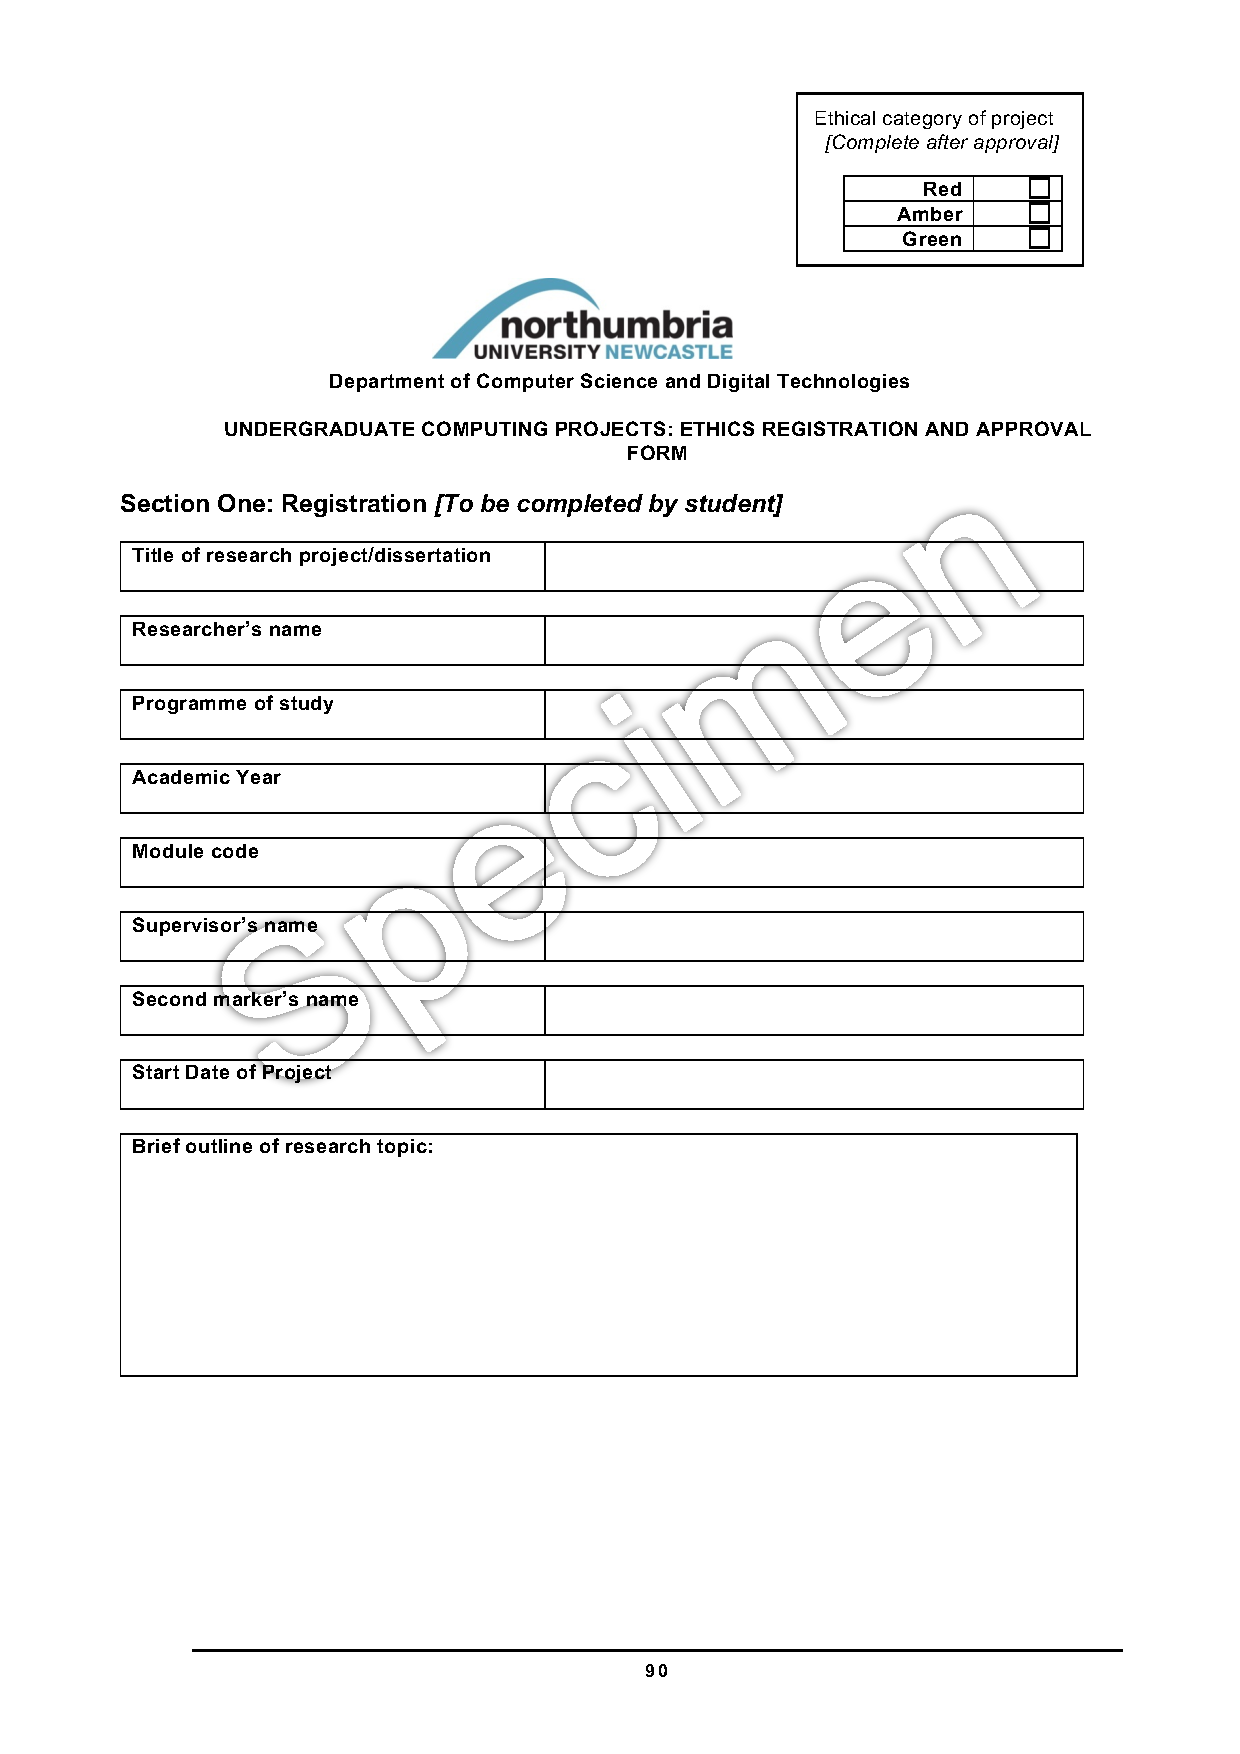
\includegraphics{ethics.pdf}
\end{tcblisting}
Assuming of course you have saved the form  as \path{ethics.pdf}

\section{Risk Assessment Form}
Likewise you can scan and include the Risk Assessment Form
\begin{tcblisting}{listing only}
\includegraphics{risk-assesment.pdf}
\end{tcblisting}

\end{document}
